
\chapter{Conclusiones}\label{cap.conclusiones}

\par Como se mencionó en el capítulo \ref{cap.introduccion} el objetivo era obtener resultados aceptables en la clasificación de la ironía en textos cortos, y por lo visto en el capítulo \ref{cap.experimentos} los resultados descritos se asemejan a los de la bibliografía y en algunos casos superan lo esperado, por lo que el objetivo puede considerarse cumplido. Sin embargo, dentro de las observaciones de mejora que se reportan está cambiar la arquitectura del modelo. Como se trato en el capitulo \ref{cap.experimentos} la tesis que se presenta se enfoca más en el preprocesamiento ya que como demuestran los resultados impacta de forma directa en el desempeño del modelo. En este proyecto se usa una arquitectura del modelo que ha reportado buen desempeño en la clasificación de reseñas de películas de IMDB. La cual es una tarea que se acerca bastante a la clasificación de la ironía, ya que se trata de extraer una opinión en ambas tareas, la cual puede ser positiva o negativa, en nuestro caso irónica o no irónica.
%%%Analizar bien los resultados después

\begin{table}[H]
	\centering
	
\begin{tabular}{|l|llll|}
\hline
\# Experimento & Accuracy &     Precision &     Recall  &   F1-score \\ \hline
Experimento 1 (palabras) &       0.9687  &       0.9092  &       0.7669  &       0.8304  \\ \hline
Experimento 2 (1-gram) &       0.9825  &       {\color{OliveGreen} 0.9552}  &       0.8662  &       0.9084  \\ \hline
Experimento 3 (2-gram) &       {\color{OliveGreen} 0.9835}  &       0.9371  &       0.8958  &       {\color{OliveGreen} 0.9157}  \\ \hline
Experimento 4 (3-gram) &       0.9338  &       0.6471  &      {\color{OliveGreen}  0.9066}  &       0.7451  \\ \hline
\end{tabular}
\caption{Tabla total de métricas.}

	\label{tab:total2}
\end{table}


\par La tarea de clasificación  de la ironía se ha llevado acabo por diferentes centros de estudio, con diferentes enfoques y justificaciones, desde los sistemas de reglas que propuso \cite{utsumi1996unified} a las técnicas modernas como arboles aleatorios \cite{lopez2016character}. Como se explico brevemente en el capítulo \ref{cap.experimentos} la tesis presente se enfoca principalmente en definir cual de los 3 enfoques de preprocesamiento se adaptan mejor a la clasificación de la ironía, y resultó que en promedio de \textit{F-score} el mejor modelo fue el del tercer experimento. %Aqui meter conclusion% 

\par A lo largo de los experimentos se pudo ver que sus métricas cambiaban bastante, debido principalmente a como se llevaba a acabo el preprocesamiento. Este preprocesamiento indicó que fue mucho mejor realizar un preprocesamiento por n-gram de dos, debido a que el \textit{F-score} es mejor que en cualquiera de los experimentos. Para retomar un poco el análisis que se realizó en los diferentes experimentos, se describirá brevemente cual fue el preprocesamiento, la configuración de la red neuronal y los resultados.

\par En el primer experimento se tomaron las palabras separadas por signos de puntuación o espacios, como tokens. A estos se les aplicó una discretización, transformándolos a un entero, el cual fue su índice en un diccionario. De este preprocesamiento se extrajeron vectores por tweet, los cuales se pasaron por una red neuronal con una configuración de una capa de embeddings, una de \gls{bi-lstm} y por último una capa totalmente conectada, de la cual se obtenía un 1 si la sentencia fue irónica y un 0 si no lo era.

\par Sus resultados fueron relativamente buenos, ya que obtuvo un promedio de \textit{F-score} de 83.04 \%. Respecto a sus medidas de \textit{precision} y \textit{recall}, este experimento tuvo 90.92 \% y 76.69 \% respectivamente.

\par En el segundo experimento se hizo un preprocesamiento llamado n-gram de 1, por caracter. En este experimento no se excluyeron los caracteres especiales. Se tuvo una configuración similar en la red neuronal, con excepción que la entrada ahora fueron vectores de 200 elementos.

\par Sus resultados fueron significativamente mejores que los del primer experimento ya que sube a 90.84 \% de \textit{F-score}. Tanto el \textit{precision} como el \textit{recall} mejoraron teniendo 95.52 \% y 86.62 \% respectivamente. Este segundo modelo se considera por los resultados mejor que el anterior en todo sentido.

\par En el tercer experimento se aumento el n-gram a 2 y se uso la misma red neuronal que la del segundo experimento.

\par Sus resultados fueron ligeramente mejores que el anterior, llegando a tener un 91.57 \% de \textit{F-score}. Sin embargo, el \textit{precision}
disminuye a 93.71 \%, pero aumenta el \textit{recall} a 89.58 \%. Por estas pequeñas diferencias se podría considerar un mejor modelo el del tercer experimento. No obstante, si se desea un modelo que reporte una menor cantidad de falsos positivos, el primer modelo sería mejor.

\par En el cuarto experimento se aumento el n-gram a 3 y se uso la misma configuración de red neuronal.

\par En cuanto a sus resultados fueron los peores de los 4 experimentos.Cayo el \textit{F-score} a 74.51 \%. Su \textit{precision} cayó a 64.71 \%. Sin embargo su \textit{recall} aumento respecto a cualquier experimento a 90.66 \% lo cual lo hace el experimento con mejor \textit{recall}. Este modelo es el peor de todos en promedio, sin embargo, si lo que se quiere es un sistema que encuentre la mayor cantidad de muestras positivas este es el mejor de todos, aunque terminará prediciendo también una gran cantidad de falsos positivos.

\par El modelo más confiable respecto a las métricas es el tercero por su  promedio de \textit{F-score}, el cual indica que es el mejor equilibrado y que aunque  no es el que tiene el mejor \textit{recall} o \textit{precision} tiene la mayor confiabilidad de los tres ya que se equivocará menos veces.

\par Cabe recalcar que estas son medidas que describen el comportamiento del modelo. Sin embargo, es posible que en algunos problemas sea mucho más importante tener un mejor \textit{precision} o un mejor \textit{recall}. Esto dependerá del uso que tenga el modelo.

\par Por todas estas razones se puede ver que el objetivo de proponer un modelo de red neuronal que pueda identificar la ironía, se ha cumplido. Debido a lo descrito el capítulo \ref{cap.experimentos} se encuentra que el \textit{F-score} promedio del experimento 3, es el mejor del los 4 experimentos que se realizaron. A pesar de que los resultados son superiores a los reportados en el capítulo \ref{cap.antecedentes}, estos no se puede comparar directamente debido a que los corpus usados en la bibliografía confiaban enteramente en que los usuarios etiquetaban correctamente los textos irónicos. Sin embargo, esto no es así siempre. Si los cálculos reportan que el porcentaje de muestras irónicas es de alrededor del 10\% se debe tener en cuenta que también este porcentaje de muestras etiquetadas como irónicas pueden aportar información confusa que impactará directamente en el desempeño, y las métricas después no podrán ser completamente fidedignas ya que no se toma en cuenta que no es la ironía lo que se está detectando, sino cuando los usuarios usarán la etiqueta de \#ironía. Como se puede ver en la figura \ref{fig:ejemploNoironia}.
\begin{figure}
	\centering
	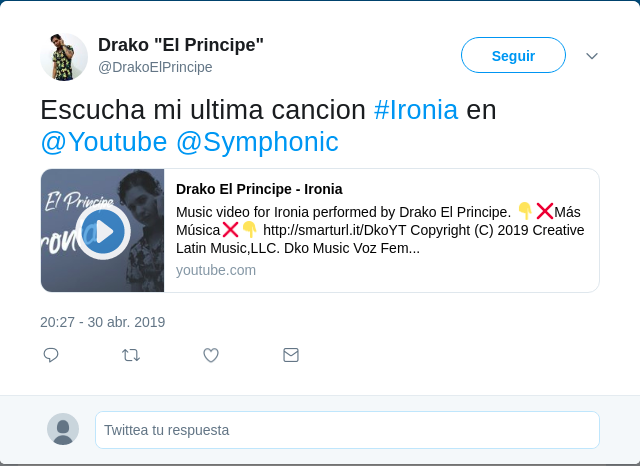
\includegraphics[width=\linewidth]{imagenes/ejemploIroniaNoironia.png}
	\caption{Ejemplo de una muestra que no esta bien etiquetada.}
	\label{fig:ejemploNoironia}
\end{figure}

\par Por esta razón no se pueden comparar los resultados extraídos en esta ocasión, ya que no hay trabajo previo con el se puedan comparar directamente. Aún así el modelo aquí propuesto  tiene un desempeño con un 98.35\% de accuracy, 93.71\% de \textit{precision}, 89.58\% de \textit{recall} y 91.57\% de \textit{F-score}, lo cual significa que el 98.35\% de las ocasiones acertará en la clasificación asignada, el 93.71\% de las muestras detectadas como irónicas son de verdad irónicas y el modelo encontrará el 89.58\% de las muestras irónicas. Dicho desempeño puede considerarse bueno ya que su \textit{F-score} supera el 80\% promedio.

\section{Trabajos a futuro}

\par Como sugerencia para trabajos posteriores se puede establecer una metodología de exploración entre los diferentes modelos que podrían dar mejores resultados. Como la combinación de la arquitectura CNN y la LSTM. Incluso se podrían explorar los nuevos algoritmos de optimización como el Artifitial Plant Optimization o algoritmos genéticos.

\par Por otro lado se pueden implementar o aumentar el preprocesamiento que se usó en este trabajo, tal vez añadiendo etiquetas POS para que éstas aporten diferentes características a la clasificación. Además de esto mi sugerencia es aumentar el tamaño del corpus para obtener una muestra más significativa de la ironía. También puede considerarse una revisión a fondo de los tweets que componen el corpus con el fin de depurar errores de concepto de ironía.

\par Además podría realizarse un estudio en el que se extraigan más clases de ironía como sarcasmo o sátira. Para obtener esto se deben tener claros los conceptos de ironía, sarcasmo y sátira, por lo que se sugiere antes de hacer un modelo que distinga de estos tres, realizar un modelo que distinga el sarcasmo de lo que no lo es, y otro que distinga la sátira de lo que no lo es. Esto sugiero se lleve acabo en un corpus con muestras irónicas y sarcásticas/satíricas con el fin de que el modelo también pueda distinguir el sarcasmo/sátira de la ironía.

\par Los textos usados en este trabajo proceden de diferentes países. Sin embargo, el idioma no se comporta de la misma manera en todos los lugares donde se habla. Por lo que otro factor a tomar en cuenta para realizar un mejor modelo que detecte mejor la ironía en español es recabar datos de igual tamaño de todos los países donde se hable este idioma. Entonces se tienen dos opciones, realizar el modelo. Por cada uno de los países realizar otro modelo que detecte de que país es el texto, un problema bastante complejo, y de este modo redirigir el texto al modelo que detecte la ironía para ese país. La otra opción es crear un modelo que tome todo el corpus de todos los países y se entrene para detectar la ironía. Si se realiza de la primera forma se tendrá una forma más certera de encontrar la ironía ya que se adaptaría el modelo a la forma de hablar en ese país. De la segunda forma se ahorraría el primer modelo que clasifique la nación, y solo se tendría que entrenar un modelo, por lo que se ahorraría tiempo. Sin embargo, dado que se usaría la misma arquitectura para detectar la ironía en diferentes países, el modelo tendería a tener un peor desempeño debido a que se entrenaría para un dialecto universal del español, el cual en la realidad no existe. Esto provocaría que se contradiga algunas veces debido a que las mismas palabras tienen diferentes significados en diferentes países.